\chapter{Présentation de l'entreprise}

\ebi{} est une société de services basée en région parisienne et appartient au \excilysGroup{} \cite{excilys}.

\section{Le \excilysGroup{}}

\excilys{} est un groupe regroupant sept sociétés de services (Adlys, Altendis, \ebi{}, Edvance, Equitalis, SS2J et Visual3X) spécialisé dans les technologies Java/JEE. Ce groupe est né du développement d'\ebi{}.

\subsection{Historique du groupe}

L'histoire de la société commence en 2000 avec la création d'\ebi{}. Cette entreprise avait pour vocation de répondre à des problématiques pointues dans le cadre de développement Java/JEE, notamment dû au fait que les grands comptes manquaient d'expertises sur ce domaine.
\ebi{} s'est placée sur cette niche de l'expertise technique en Java/JEE, dans le secteur de l'assurance puis graduellement dans d'autres secteurs d’activités (Santé, Banque, Sécurité, Fret…).\\

En 2002, l’entreprise a décidé de refondre son organisation interne, que ce soit au niveau de la gestion des rémunérations, la gestion des carrières ou le recrutement. Ce remaniement profond a donné naissance à la charte \excilys{} (cf. annexe~\ref{ann:charte}).
Cette charte définit des règles que la société s'impose envers ses clients et ses consultants. Elle définit un modèle pour la prestation de service : le Service Équitable.\\

Les résultats probants de cette démarche ont poussé l'entreprise à se développer en proposant ce modèle à d'autres sociétés de services voulant se spécialiser dans l'excellence technique. \excilys{} est né.

\subsection{La société \ebi{}}

\ebi{} se concentre toujours dans l'expertise technique dans le domaine Java/JEE en proposant conseils et développements à ses clients.
La société intervient également en tant que sous-traitant de grandes sociétés de services pour définir l'architecture de leur projet tout en encadrant leurs équipes.
La société, étant experte sur un domaine, s'est logiquement dirigée vers le coaching et l'organisation de formations.\\

Elle propose en effet des cycles de formation complets (Java Academy), des audits d'infrastructures, l'implantation de solution Open Source ou encore de l'assistance à maîtrise d'ouvrage dans le cadre d'un développement d'applications JEE.\\

\begin{figure}[H]
	\centering
	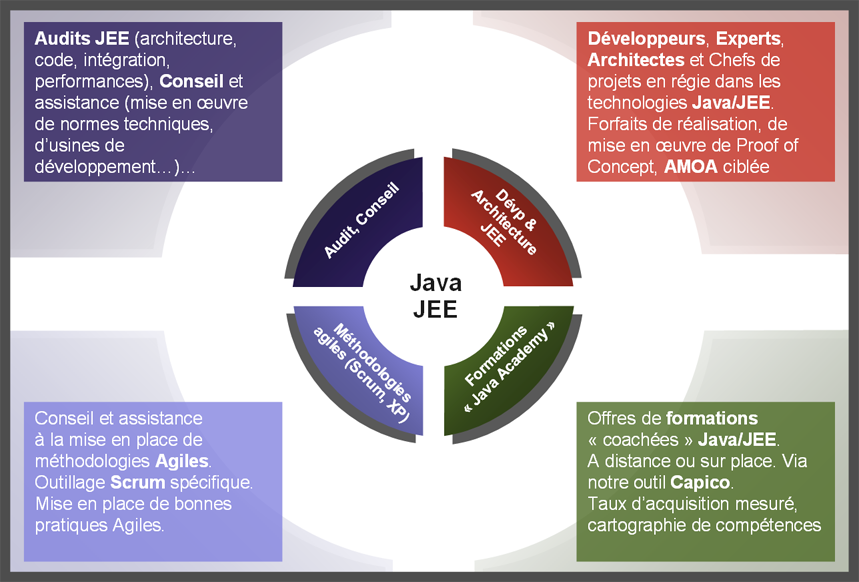
\includegraphics[width=\linewidth]{images/diag_metier.pdf}
	\caption{Les 4 métiers}
\end{figure}


Compte tenu des bons résultats de l'entreprise, elle dispose désormais de nombreux clients, dans de multiples secteurs d'activités.\\

\begin{figure}[H]
	\centering
	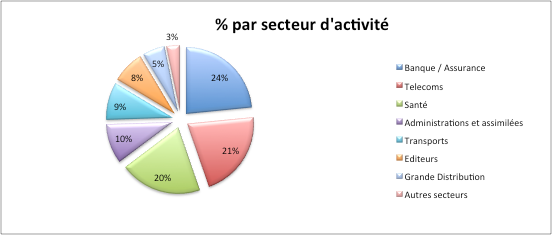
\includegraphics[width=\linewidth]{images/pie_ca.pdf}
	\caption{Répartition du chiffre d'affaires par secteur d'activité}
\end{figure}

En 2009, \ebi{} a décidé d'élargir son pôle de compétences en investissant notamment sur les plateformes mobiles Android, puis sur des plateformes iOS (iPhone) en 2010. Elle a aussi décidé de monter en compétences dans un secteur porteur : le cloud, notamment AppEngine (Google) et Amazon EC2 et S3.\\

Au niveau économique, \ebi{}  est une SARL ne disposant d'aucun investisseur financier externe. Son chiffre d'affaires est en constante augmentation jusqu'en 2008, puis en diminution en 2009 : conséquence de la crise financière. Il retrouve finalement un niveau équivalent à 2008 en 2010 avec un chiffre d'affaires hors taxe de 7.4 M\euro{}.\\

\begin{figure}[H]
	\centering
	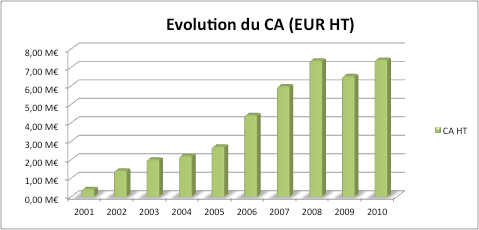
\includegraphics[width=\linewidth]{images/diag_ca.pdf}
	\caption{Évolution du chiffre d'affaires}
\end{figure}

\subsection{Les autres entités du groupe}

En plus d'\ebi{}, le groupe compte six autres sociétés respectant la charte \excilys{} dans des domaines similaires :

\begin{description}
	\item [Altendis] 
	Spécialisée dans le développement Java/JEE avec des profils moins expérimentés que ceux d'\ebi{}, la société offre des prestations essentiellement dans des projets de développements. Cette société emploie directement les stagiaires en fin de stage.
	
	\item [SS2J] 
	Spécialisée autour de la conduite de projets, la société offre des prestations dans le domaine du coaching, la gestion de projets en suivant les méthodes agiles.
	
	\item [Edvance] 
	La société est spécialisée dans les solutions autour de la technologie RFID (\textit{Radio Frequency IDentifier}). La société est partenaire de STMicroElectronics et offre parmi ses solutions, un système complet de gestion des accès à un bâtiment par contrôle RFID/JEE des personnes.
	
	\item [Equitalis]
	L'entreprise est située à Bordeaux. Equitalis propose des prestations similaires à \ebi{} (architecture JEE, gestion de projets Agile, formation et coaching). Elle est la première société basée en province respectant la charte \excilys{}.
	
	\item [Adlys]
	Adlys est une société de conseil, d'ingénierie et de formation, spécialisée dans les infrastructures Java/JEE qui a notamment apporté son expérience dans le domaine du coaching et de la formation aux autres sociétés du groupe.
	
	\item [Visual3X] 
	Visual3X est la société spécialisée dans la mise en place de clients riches et d'interface Web 2.0 et propose du conseil, de la formation ou du développement. 
\end{description}

\section{L'organisation de l'entreprise}

\ebi{} étant détenue intégralement par ses dirigeants, l'entreprise reste maître de son évolution et de son fonctionnement, en restant régie par la charte \excilys{}.

\subsection{Le service équitable - La charte \excilys{}}

La charte \excilys{} est une action assez unique en son genre dont le but est de prôner certaines valeurs pour assurer une meilleure implication des consultants chez leurs clients. Ceci passe par un salaire du consultant proportionnel à la facturation cliente et des consultants adaptés à la mission.

\begin{figure}[H]
	\centering
	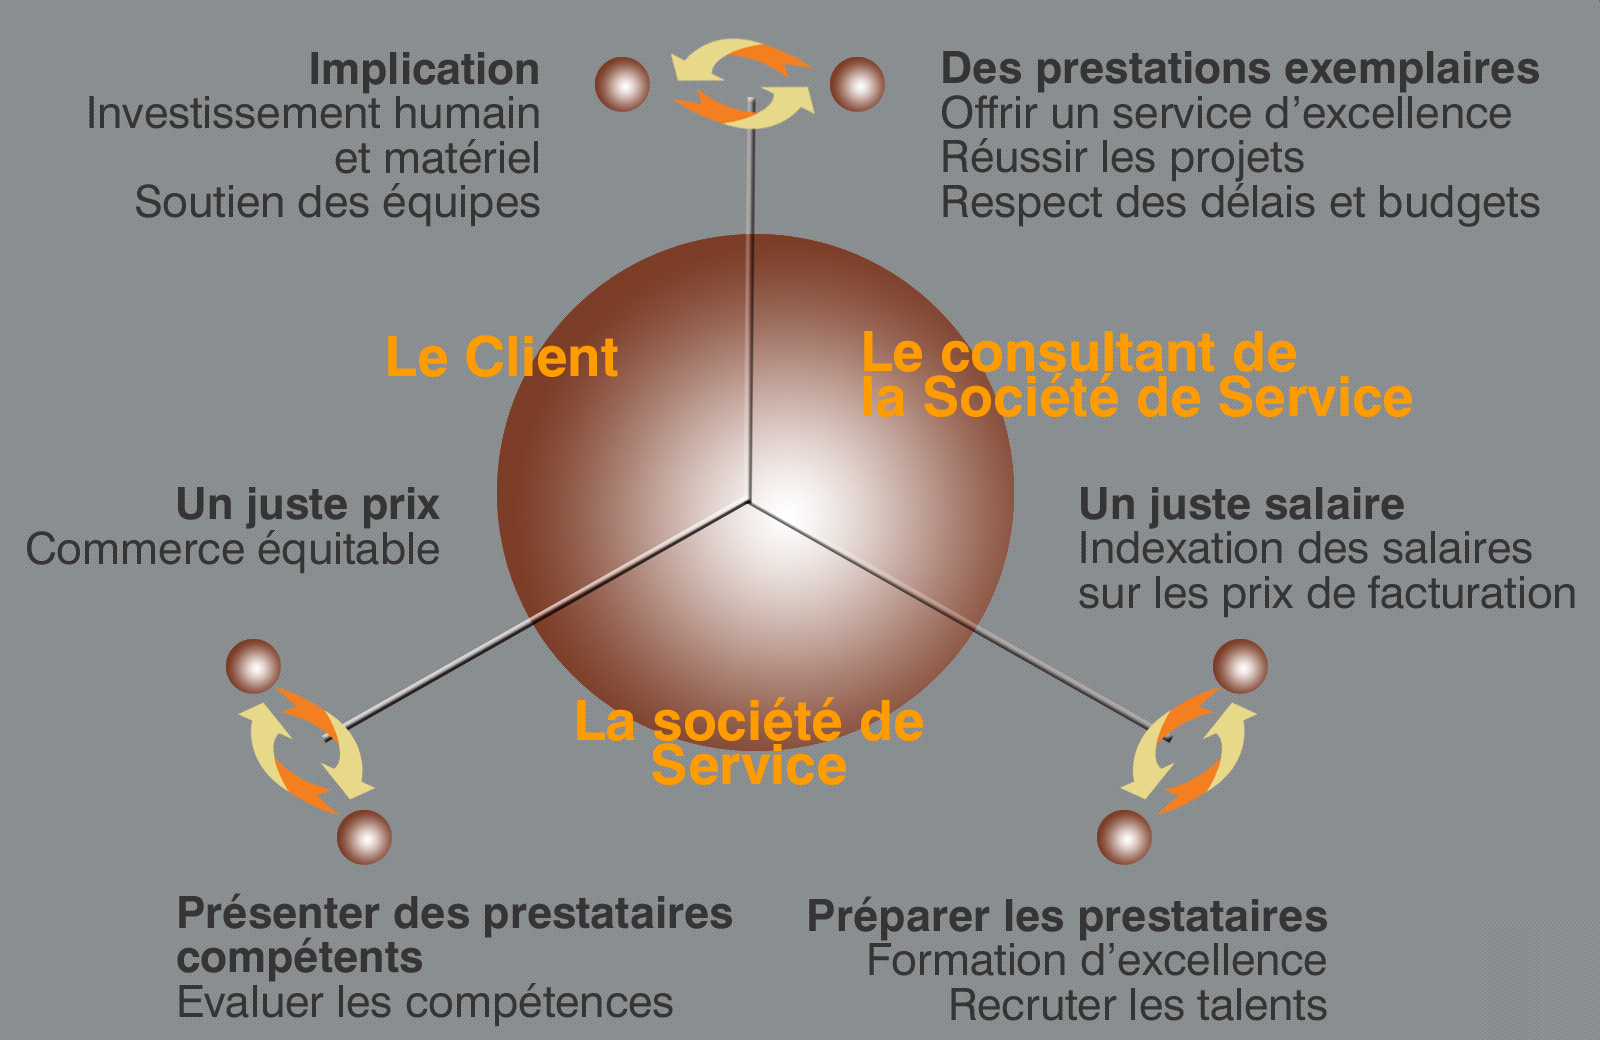
\includegraphics[width=\linewidth]{images/diag_equi.pdf}
	\caption{Le service équitable}
\end{figure}

Pour préparer les consultants, \ebi{} s'appuie sur des formations et le partage de connaissances qui est un des aspects les plus importants pour \excilys{} car il permet une montée en compétence rapide de ses consultants. Pour mener à bien cette action, un système de capitalisation de compétences, \capico{} \cite{capico}, développé en interne, a été mis en place.

\subsection{Le système d'information du groupe}

Le système d'information du groupe \excilys{}, est composé de différents modules : 

\begin{itemize}
	\item Les modules fonctionnels 
	\item Les modules techniques
	\item La gestion des droits\\
\end{itemize}

Les modules fonctionnels correspondent à tous les outils permettant de gérer la plupart des problématiques pour l'entreprise, c’est-à-dire tous les aspects de gestion commerciale mais également la gestion des compétences et des connaissances ou encore les aspects communications (Mail ,site internet , blog, forum,\ldots). Les aspects administratifs sont également gérés via une application développée en interne, Maestro.\\

Les modules techniques servent de support aux modules fonctionnels.
Finalement, la gestion des droits permet de gérer, via le module Security, les accès aux différents modules.
A terme, l'ensemble des services sera géré via un ESB(\textit{Entreprise Service Bus}).
Les stages effectués chez \ebi{} se déroule généralement sur une partie du système d'information, notamment dans les modules fonctionnels.

\begin{figure}[H]
	\centering
	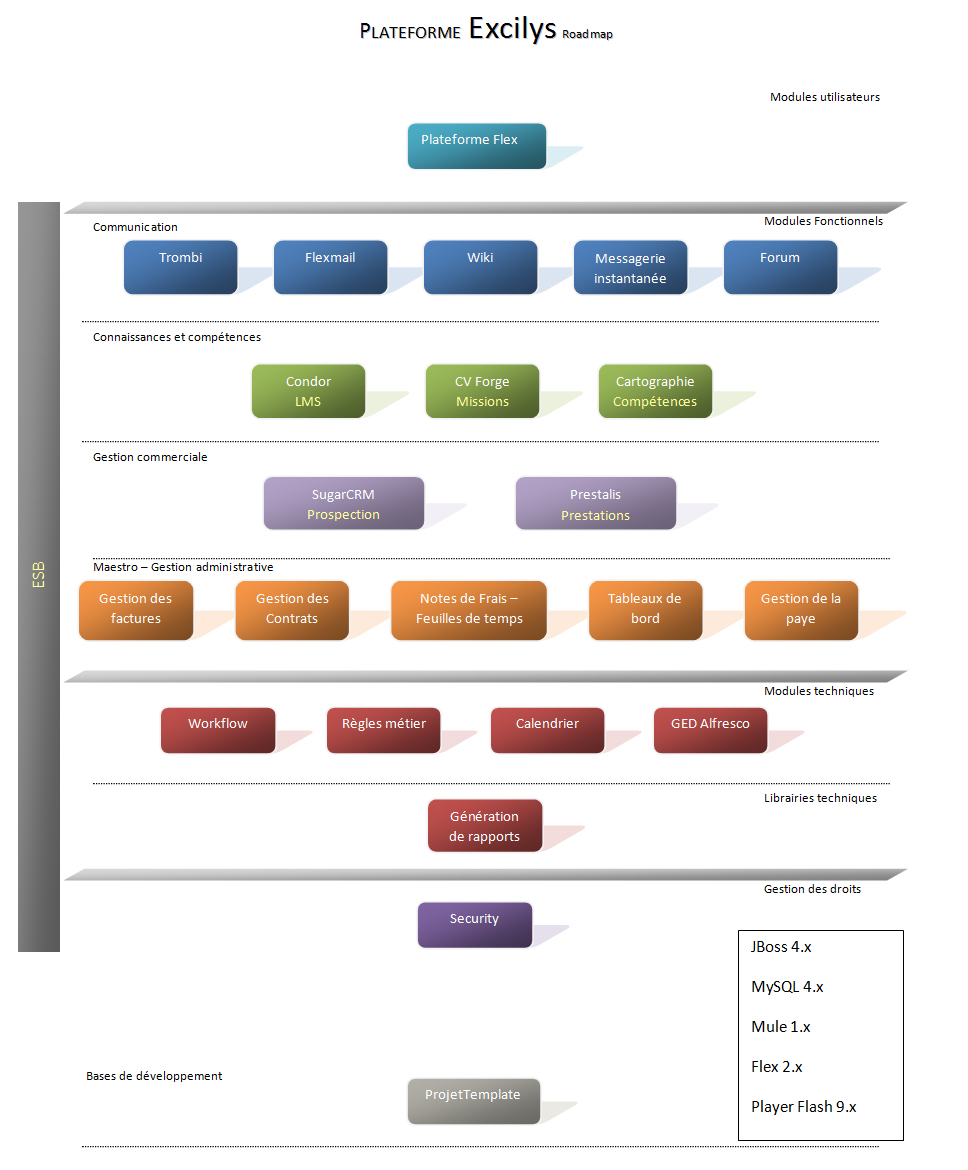
\includegraphics[width=\linewidth]{images/diag_si.pdf}
	\caption{Système d'information du groupe \excilys{}}
\end{figure}
